% !TeX program = xelatex
\documentclass[a4paper,10pt]{article}

% ============================================================================
% សន្លឹកកិច្ចការសិស្សបំពេញចន្លោះ ស-ខ្មៅ និងប្លង់ក្ដារខៀន/ចម្លើយគ្រូ (គ្មាន LCD / គ្មានកន្ត្រៃ)
% មេរៀនទី៥ (២.១--២.៣)៖ សញ្ញាណពហុធា ដឺក្រេ និងវិធីបូកដកពហុធា — ត្រូវគ្នានឹង LS_Plan_ALG53.tex
% ============================================================================
\usepackage[a4paper, left=1.0cm, right=1.0cm, top=0.75cm, bottom=1.00cm, footskip=0.52cm]{geometry}
\usepackage{amsmath}
\usepackage{unicode-math}
\usepackage{fontspec}
\usepackage{array, colortbl}
\usepackage[table]{xcolor}
\usepackage{enumitem}
\usepackage{pifont}
\usepackage{fancyhdr}
\usepackage{lastpage}
\usepackage{tikz}
\usepackage[most]{tcolorbox}
\usetikzlibrary{calc, arrows.meta, decorations.pathreplacing, positioning, babel}

\makeatletter
\let\@expl@@@mark@update@singlecol@structures@@\relax
\makeatother

\providecommand{\NGSFindFonts}{%
  \IfFileExists{C:/Windows/Fonts/cambria.ttc}{%
    \def\NGSSysPath{C:/Windows/Fonts/}%
    \def\NGSUserPath{C:/Users/KIT/AppData/Local/Microsoft/Windows/Fonts/}%
  }{%
    \IfFileExists{./fonts/KhmerOSsiemreap.ttf}{\def\NGSSysPath{./fonts/}\def\NGSUserPath{./fonts/}}{%
    \IfFileExists{../fonts/KhmerOSsiemreap.ttf}{\def\NGSSysPath{../fonts/}\def\NGSUserPath{../fonts/}}{%
    \IfFileExists{../../fonts/KhmerOSsiemreap.ttf}{\def\NGSSysPath{../../fonts/}\def\NGSUserPath{../../fonts/}}{%
    \IfFileExists{../../../fonts/KhmerOSsiemreap.ttf}{\def\NGSSysPath{../../../fonts/}\def\NGSUserPath{../../../fonts/}}{%
    \IfFileExists{../../../../fonts/KhmerOSsiemreap.ttf}{\def\NGSSysPath{../../../../fonts/}\def\NGSUserPath{../../../../fonts/}}{%
    \IfFileExists{../../../../../fonts/KhmerOSsiemreap.ttf}{\def\NGSSysPath{../../../../../fonts/}\def\NGSUserPath{../../../../../fonts/}}{%
    \IfFileExists{../../../../../../fonts/KhmerOSsiemreap.ttf}{\def\NGSSysPath{../../../../../../fonts/}\def\NGSUserPath{../../../../../../fonts/}}{%
      \def\NGSSysPath{../../../../../../../fonts/}\def\NGSUserPath{../../../../../../../fonts/}%
    }}}}}}}%
  }%
}
\NGSFindFonts

\setmathfont[Path={\NGSSysPath}, FontIndex=1, Scale=1.02]{cambria.ttc}
\defaultfontfeatures{Ligatures=TeX}

\setmainfont[
  Path={\NGSUserPath}, Extension=.ttf, Script=Khmer,
  BoldFont={KhmerOSsiemreap}, BoldFeatures={FakeBold=1.8},
  ItalicFont={KhmerOSsiemreap}, ItalicFeatures={FakeSlant=0.25},
  BoldItalicFont={KhmerOSsiemreap}, BoldItalicFeatures={FakeBold=1.8, FakeSlant=0.25}
]{KhmerOSsiemreap}

\newfontfamily\muol[Path={\NGSUserPath}, Extension=.ttf, Script=Khmer]{KhmerOSmuollight}
\newfontfamily\TimesEn[Path={\NGSSysPath}, Extension=.ttf, BoldFont={timesbd}, ItalicFont={timesi}, BoldItalicFont={timesbi}]{times}
\newfontfamily\CalibriFont[Path={\NGSSysPath}, Extension=.ttf]{calibri}

\XeTeXlinebreaklocale "km"
\XeTeXlinebreakskip = 0pt plus 1pt minus 0.1pt

\definecolor{panelgray}{gray}{0.94}
\definecolor{headgray}{gray}{0.85}

\pagestyle{fancy}
\fancyhf{}
\renewcommand{\headrulewidth}{0pt}
\fancyfoot[L]{\fontsize{7.4pt}{9.5pt}\selectfont អនុវិទ្យាល័យព្រះក្រសាំង \en{|} គ្រូ៖ ហុក ប៊ុនថែន \en{|} មេរៀនទី៥ (២.១--២.៣) ពហុធានិងបូកដកពហុធា \en{|} ថ្ងៃចន្ទ ទី៧ ខែធ្នូ ឆ្នាំ២០២៦}
\fancyfoot[R]{\fontsize{7.8pt}{10pt}\selectfont ទំព័រ \en{\thepage\ / \pageref{LastPage}}}

\setlength{\parindent}{0pt}
\setlength{\parskip}{0pt}
\setlength{\tabcolsep}{4pt}

\newcommand{\en}[1]{{\TimesEn #1}}
\newcommand{\enbf}[1]{{\TimesEn\bfseries #1}}
\newcommand{\unit}[1]{\,\text{\en{#1}}}
\newcommand{\riel}{\,\text{៛}}
\newcommand{\cnum}[1]{\mbox{\fontsize{10pt}{12pt}\selectfont\ding{\numexpr181+#1\relax}}}
\newcommand{\chkbox}{\tikz[baseline=-0.15ex]\draw[black, line width=0.85pt, fill=white] (0,0) rectangle (0.24cm,0.24cm);}
\newcommand{\ansbox}[1][2.0cm]{\,\tikz[baseline=-0.65ex]\draw[black, line width=0.65pt, fill=white] (0,0) rectangle (#1, 0.42cm);\,}
\newcommand{\dotline}[1][2.2cm]{\makebox[#1]{\dotfill}}

\newcommand{\pagebanner}[2]{%
  \begin{tcolorbox}[
    enhanced, sharp corners, colback=headgray, colframe=black,
    boxrule=1.05pt, boxsep=1pt, top=2.5pt, bottom=2.5pt, left=6pt, right=6pt,
    after skip=3.5pt
  ]
    {\muol\fontsize{9.0pt}{13.2pt}\selectfont #1}\hfill{\fontsize{8.0pt}{11.2pt}\selectfont\textbf{#2}}
  \end{tcolorbox}%
}

\newcommand{\secstrip}[2]{%
  \vspace{3pt}%
  \begin{tcolorbox}[
    enhanced, sharp corners, colback=panelgray, colframe=black,
    boxrule=0.8pt, boxsep=0.8pt, top=2pt, bottom=2pt, left=5pt, right=5pt,
    after skip=3pt
  ]
    {\muol\fontsize{8.5pt}{12.2pt}\selectfont #1}\hfill{\fontsize{7.8pt}{10.8pt}\selectfont\textit{#2}}
  \end{tcolorbox}%
}

\newcolumntype{L}[1]{>{\raggedright\arraybackslash}p{#1}}
\newcolumntype{C}[1]{>{\centering\arraybackslash}p{#1}}

\begin{document}
\fontsize{9.5pt}{14.5pt}\selectfont

% ============================================================================
% ទំព័រទី ១៖ សន្លឹកកិច្ចការសិស្ស (ផ្នែកមុខ៖ E1 -> E2 -> E3)
% ============================================================================
\pagebanner{សន្លឹកកិច្ចការសិស្ស \enbf{(}៥\enbf{.}២\enbf{.}១\enbf{--}៥\enbf{.}២\enbf{.}៣ ពហុធានិងបូកដកពហុធា\enbf{)} \enbf{--} ផ្នែកមុខ}{ថ្នាក់ទី៨ \en{|} សៀវភៅគោល ទំ.៥៦--៥៩}

\begin{tcolorbox}[
  enhanced, sharp corners, colback=white, colframe=black,
  boxrule=0.8pt, boxsep=1.5pt, top=3.5pt, bottom=3.5pt, left=5pt, right=5pt,
  after skip=4pt
]
  \fontsize{9.0pt}{13.0pt}\selectfont
  \textbf{ឈ្មោះសិស្ស៖} \dotline[4.3cm] \quad
  \textbf{សមាជិកក្រុម៖} \dotline[4.3cm] \quad
  \textbf{ថ្នាក់ទី៖} ៨\dotline[0.9cm] \quad
  \textbf{ក្រុមទី៖} \dotline[1.0cm]
\end{tcolorbox}

% --- E1 Engage ---
\secstrip{ផ្នែកទី ១ \enbf{(E1 - Engage)} ៖ បេសកកម្មអន្ទាក់សញ្ញាដកមុខវង់ក្រចក}{រយៈពេល ៣ នាទី (គូស \ding{51} ក្នុង \chkbox)}

\begin{tcolorbox}[
  enhanced, sharp corners, colback=white, colframe=black,
  boxrule=0.8pt, boxsep=2.5pt, top=4pt, bottom=4pt, left=6pt, right=6pt
]
  គេឱ្យផលដកពហុធា $(3x^2 - 2x + 7) - (x^2 + 4x + 5)$ ។ តើសិស្សរូបណាគណនាបានត្រឹមត្រូវ?\\[3pt]
  \chkbox\ \textbf{សិស្ស ក៖} $3x^2 - 2x + 7 - x^2 + 4x + 5 = 2x^2 + 2x + 12$ \qquad
  \chkbox\ \textbf{សិស្ស ខ៖} $3x^2 - 2x + 7 - x^2 - 4x - 5 = 2x^2 - 6x + 2$\\[3pt]
  $\bullet$ \textbf{ហេតុផលខ្លី៖} ពេលលុបវង់ក្រចកក្រោយសញ្ញាដក $-(x^2 + 4x + 5)$ គេបាន $-x^2$ \dotline[1.6cm] \dotline[1.6cm] ។
\end{tcolorbox}

\vspace{3pt}

% --- E2 Explore ---
\secstrip{ផ្នែកទី ២ \enbf{(E2 - Explore)} ៖ សញ្ញាណពហុធា ដឺក្រេ និងវិធីបូកដកពហុធា (ទំ.៥៦--៥៩)}{រយៈពេល ១១ នាទី}

\textbf{សកម្មភាព ១ (\en{E2-A} — ៥ នាទី)៖ សញ្ញាណពហុធា និងដឺក្រេនៃពហុធា (ទំ.៥៦--៥៨)}

\begin{tcolorbox}[
  enhanced, sharp corners, colback=white, colframe=black,
  boxrule=0.8pt, boxsep=2.5pt, top=4pt, bottom=4pt, left=6pt, right=6pt
]
  \begin{minipage}[c]{4.0cm}
    \centering
    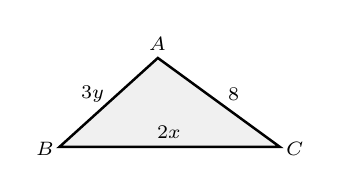
\begin{tikzpicture}[x=1cm, y=1cm, every node/.style={font=\scriptsize, text=black}]
      \draw[black, line width=0.9pt, fill=gray!12] (0.2,0.15) -- (3.0,0.15) -- (1.45,1.28) -- cycle;
      \node at (0.02,0.12) {$B$};
      \node at (3.18,0.12) {$C$};
      \node at (1.45,1.46) {$A$};
      \node at (0.62,0.82) {$3y$};
      \node at (2.42,0.82) {$8$};
      \node at (1.60,0.34) {$2x$};
    \end{tikzpicture}
  \end{minipage}\hfill
  \begin{minipage}[c]{14.0cm}
    $\bullet$ \textbf{១) បរិមាត្រត្រីកោណ $ABC$ (ទំ.៥៦)៖} $AB + BC + CA =$ \dotline[3.6cm] ហៅថា \textbf{ពហុធា} ។\\[3pt]
    $\bullet$ \textbf{២) ឈ្មោះតាមចំនួនតួ៖} ពហុធា $3x - 8$ មាន $2$ តួ ហៅថា \dotline[2.0cm]; \ ឯ $5x^2 - 2x + 7$ មាន $3$ តួ ហៅថា \dotline[2.0cm] ។\\[3pt]
    $\bullet$ \textbf{៣) ដឺក្រេ និងលំដាប់ (ទំ.៥៧--៥៨)៖} ពហុធា $11 + 5x^2 - 3x$ មានដឺក្រេ \ansbox[1.2cm] រៀបតាមលំដាប់\textbf{ចុះ}បាន \dotline[3.6cm] ។
  \end{minipage}
\end{tcolorbox}

\vspace{4pt}
\textbf{សកម្មភាព ២ (\en{E2-B} — ៦ នាទី)៖ វិធីបូក និងដកពហុធាតាមជួរដេក និងជួរឈរ (ទំ.៥៨--៥៩)}

\begin{tcolorbox}[
  enhanced, sharp corners, colback=white, colframe=black,
  boxrule=0.8pt, boxsep=2.5pt, top=4pt, bottom=4pt, left=6pt, right=6pt
]
  $\bullet$ \textbf{១) គណនាជួរដេក (ទំ.៥៨)៖} បើ $A = 2a^2 + 3a - 4$ និង $B = 5a^2 - 7a + 6$ នោះ៖\\[2pt]
  \hspace*{0.3cm}$A + B = (2a^2 + 5a^2) + (3a - 7a) + (-4 + 6) =$ \ansbox[4.2cm]\\[4pt]
  $\bullet$ \textbf{២) គណនាជួរឈរ (លំហាត់គំរូ ទំ.៥៨--៥៩)៖} បើ $A = 5x^3 - 2x^2 + 7x + 4$ និង $B = 2x^3 + 4x^2 - 6$ (ថែមតួ $0x$)៖\\[2pt]
  \hspace*{0.3cm}-- ផលបូក $A + B =$ \ansbox[4.8cm] \qquad
  -- ផលដក $A - B =$ \ansbox[4.8cm]
\end{tcolorbox}

\vfill

% --- E3 Explain ---
\secstrip{ផ្នែកទី ៣ \enbf{(E3 - Explain)} ៖ និយមន័យគោល និងធនាគារហេតុផល \enbf{B\&W}}{រយៈពេល ៦ នាទី}

\begin{tcolorbox}[
  enhanced, sharp corners, colback=white, colframe=black,
  boxrule=0.85pt, boxsep=2.5pt, top=4pt, bottom=4pt, left=6pt, right=6pt
]
  $\bullet$ \textbf{១) ពហុធា៖} ជាផលបូកនៃពីរ ឬច្រើនឯកធា \dotline[2.4cm] ។ \quad
  \textbf{២) ដឺក្រេនៃពហុធា៖} ជាដឺក្រេរបស់តួដែលមានដឺក្រេ \dotline[2.6cm] ។\\[3pt]
  $\bullet$ \textbf{៣) បូក/ដកពីរពហុធា៖} លុបវង់ក្រចកឱ្យត្រូវសញ្ញា រួចបូកឬដក \dotline[3.4cm] ។\\[4pt]
  \tikz\draw[black, dashed, line width=0.5pt] (0,0) -- (18.4cm,0);\\[3pt]
  \fontsize{8.8pt}{13.0pt}\selectfont
  \textbf{ធនាគារហេតុផល (\en{Warrant Bank})៖} \quad
  \cnum{1} គ្រប់តួត្រូវជាឯកធា ($x+\frac{3}{b^2}$ មិនមែនពហុធា) \quad
  \cnum{2} ដឺក្រេពហុធា $=$ ដឺក្រេតួខ្ពស់ជាងគេ\\
  \cnum{3} ដកពហុធា៖ ប្ដូរសញ្ញាគ្រប់តួក្នុងវង់ក្រចកក្រោយសញ្ញាដក \quad
  \cnum{4} ជួរឈរ៖ ដាក់ឯកធាដូចគ្នាឱ្យចំខ្ទង់ (ថែម $0x^k$)
\end{tcolorbox}

% ============================================================================
% ទំព័រទី ២៖ សន្លឹកកិច្ចការសិស្ស (ផ្នែកខាងខ្នង៖ E4 -> E5 -> កិច្ចការផ្ទះ)
% ============================================================================
\clearpage
\pagebanner{សន្លឹកកិច្ចការសិស្ស \enbf{(}៥\enbf{.}២\enbf{.}១\enbf{--}៥\enbf{.}២\enbf{.}៣ ពហុធានិងបូកដកពហុធា\enbf{)} \enbf{--} ផ្នែកខាងខ្នង}{ថ្នាក់ទី៨ \en{|} សៀវភៅគោល ទំ.៥៧--៥៩, ៧២--៧៣}

% --- E4 Elaborate ---
\secstrip{ផ្នែកទី ៤ \enbf{(E4 - Elaborate)} ៖ លំហាត់គំរូរៀបលំដាប់ពហុធា និងគណនា \enbf{M + N, M - N} (ទំ.៥៧--៥៩)}{រយៈពេល ១០ នាទី}

\begin{tcolorbox}[
  enhanced, sharp corners, colback=white, colframe=black,
  boxrule=0.8pt, boxsep=2.5pt, top=4pt, bottom=4pt, left=6pt, right=6pt
]
  \textbf{១) បំពេញតារាងអថេរ ដឺក្រេ និងការរៀបលំដាប់កើន/ចុះ (លំហាត់គំរូ ទំ.៥៧--៥៨)៖}\\[4pt]
  {\renewcommand{\arraystretch}{1.38}
  \begin{tabular}{|C{3.8cm}|C{1.8cm}|C{1.6cm}|C{4.9cm}|C{4.9cm}|}
    \hline
    \cellcolor{headgray}\textbf{ពហុធា} & \cellcolor{headgray}\textbf{អថេរ} & \cellcolor{headgray}\textbf{ដឺក្រេ} & \cellcolor{headgray}\textbf{រៀបតាមលំដាប់កើន} & \cellcolor{headgray}\textbf{រៀបតាមលំដាប់ចុះ} \\ \hline
    $2k^3 - 4 + k^2 - k$ & $k$ & \dotline[1.0cm] & \dotline[4.2cm] & \dotline[4.2cm] \\ \hline
    $y^3 + 4y^4x + 7 + y$ & \dotline[1.3cm] & \dotline[1.0cm] & $7 + y + y^3 + 4y^4x$ & \dotline[4.2cm] \\ \hline
  \end{tabular}}\\[5pt]
  \textbf{២) ប្រតិបត្តិទំ.៥៩ (ក)៖} ឱ្យ $M = 2x^2 + 3x + 1$ និង $N = -x^2 + 2x + 4$ ។ គណនា៖\\[3pt]
  \hspace*{0.3cm}$\bullet$ $M + N =$ \ansbox[4.6cm] \qquad\qquad
  $\bullet$ $M - N =$ \ansbox[4.6cm]\\[3pt]
  \fontsize{8.8pt}{13.0pt}\selectfont
  \textbf{ឆ្លុះបញ្ចាំង (\en{EIA Looking-Back})៖} ហេតុអ្វីពហុធា $y^3 + 4y^4x + 7 + y$ មានដឺក្រេស្មើ $5$ មិនមែនស្មើ $4$? \textbf{ព្រោះ} \dotline[4.8cm] ។
\end{tcolorbox}

\vspace{4pt}

% --- E5 Evaluate ---
\secstrip{ផ្នែកទី ៥ \enbf{(E5 - Evaluate)} ៖ ប្រតិបត្តិ (ទំ.៥៧--៥៩) សំណួរវិនិច្ឆ័យ \enbf{A--D} និងសំបុត្រចេញ}{រយៈពេល ១០ នាទី}

\begin{tcolorbox}[
  enhanced, sharp corners, colback=white, colframe=black,
  boxrule=0.8pt, boxsep=2.5pt, top=4pt, bottom=4pt, left=6pt, right=6pt
]
  \textbf{១) ប្រតិបត្តិ (ទំ.៥៧ ក និង ទំ.៥៨ គ)៖} ពហុធា $6x^3 + 2xy - 4$ មានអថេរ \dotline[1.6cm] ចំនួនតួ \dotline[1.2cm]; \ ឯ $a^2 + 2ab + c^2d$ មានដឺក្រេ \ansbox[1.4cm] ។\\[4pt]
  \textbf{២) ប្រតិបត្តិទំ.៥៩ (ខ)៖} ឱ្យ $M = 12a^2 + 2ab + 54$ និង $N = 9a^2 - 4ab - 25$ ។ គណនា៖\\[3pt]
  \hspace*{0.3cm}$\bullet$ $M + N =$ \ansbox[4.8cm] \qquad\qquad
  $\bullet$ $M - N =$ \ansbox[4.8cm]\\[4pt]
  \textbf{៣) បិទបេសកកម្ម \en{E1}៖} សិស្ស \dotline[1.0cm] ត្រឹមត្រូវ ព្រោះ $(3x^2-2x+7)-(x^2+4x+5) =$ \ansbox[3.8cm] ។
\end{tcolorbox}

\vspace{4pt}

\begin{tcolorbox}[
  enhanced, sharp corners, colback=white, colframe=black,
  boxrule=0.8pt, boxsep=2.5pt, top=4pt, bottom=4pt, left=6pt, right=6pt
]
  \textbf{៤) សំណួរវិនិច្ឆ័យ \en{A--D} (គណនា $(4x^2 - 3x + 1) - (x^2 - 5x + 4)$ — គូសរង្វង់ រួចលើកម្រាមដៃ ១--៤)៖}\\[3pt]
  \textbf{\en{A.}} $3x^2 - 8x + 5$ \qquad
  \textbf{\en{B.}} $3x^2 + 2x - 3$ \qquad
  \textbf{\en{C.}} $5x^2 - 8x + 5$ \qquad
  \textbf{\en{D.}} $3x^2 - 8x - 3$\\[4pt]
  \tikz\draw[black, dashed, line width=0.5pt] (0,0) -- (18.4cm,0);\\[3pt]
  \textbf{៥) សំបុត្រចេញ ៦០ វិនាទី៖} ពហុធា $-3x^2y + \dfrac{1}{2}y^4 - 2$ មានចំនួន \ansbox[1.5cm] តួ និងមានដឺក្រេស្មើ \ansbox[1.5cm] ។
\end{tcolorbox}

\vfill

% --- Homework ---
\begin{tcolorbox}[
  enhanced, sharp corners, colback=panelgray, colframe=black,
  boxrule=0.95pt, boxsep=2pt, top=3.5pt, bottom=3.5pt, left=6pt, right=6pt
]
  {\muol\fontsize{9.0pt}{13.0pt}\selectfont កិច្ចការផ្ទះ \enbf{(}សៀវភៅគោល ទំ.៥៩ និង ទំ.៧២--៧៣ លេខ ៤, ៥ ខ\enbf{)}}\\[2.5pt]
  \fontsize{8.8pt}{13.0pt}\selectfont
  $\bullet$ \textbf{១) ប្រតិបត្តិទំ.៥៩ (គ)៖} គណនា $M+N$ និង $M-N$ បើ $M = \dfrac{1}{2}xy^2 + 2xy - 3$ និង $N = \dfrac{3}{2}xy^2 - 12xy - 16$ ។\\
  $\bullet$ \textbf{២) ទំ.៧២ \#4 និង ទំ.៧៣ \#5 ខ៖} ឱ្យ $A = 2x^2+x^4-3x+1, B = x^2-3x^3-2x^4-x+3$ គណនា $A-B, B-A$; និង $(5a^3b^2-3ab)+(2a^3b^2-ab)$ ។
\end{tcolorbox}

% ============================================================================
% ទំព័រទី ៣៖ ទំព័រគ្រូបង្រៀន (គំរូប្លង់ក្ដារខៀន ៣ ផ្នែក + ចម្លើយផ្ទៀងផ្ទាត់រហ័ស)
% ============================================================================
\clearpage
\pagebanner{ទំព័រគ្រូបង្រៀន ៖ ប្លង់ក្ដារខៀន \enbf{(}គ្មាន \enbf{LCD)} និងចម្លើយផ្ទៀងផ្ទាត់រហ័ស}{៥.២.១--៥.២.៣ ពហុធានិងបូកដកពហុធា (\en{ALG53})}

\secstrip{១. គំរូប្លង់បែងចែកក្ដារខៀន ៣ ផ្នែក សម្រាប់ថ្នាក់រៀនគ្មាន \enbf{LCD}}{សម្រាប់គ្រូប្រើដីស/ហ្វឺត}

\begin{center}
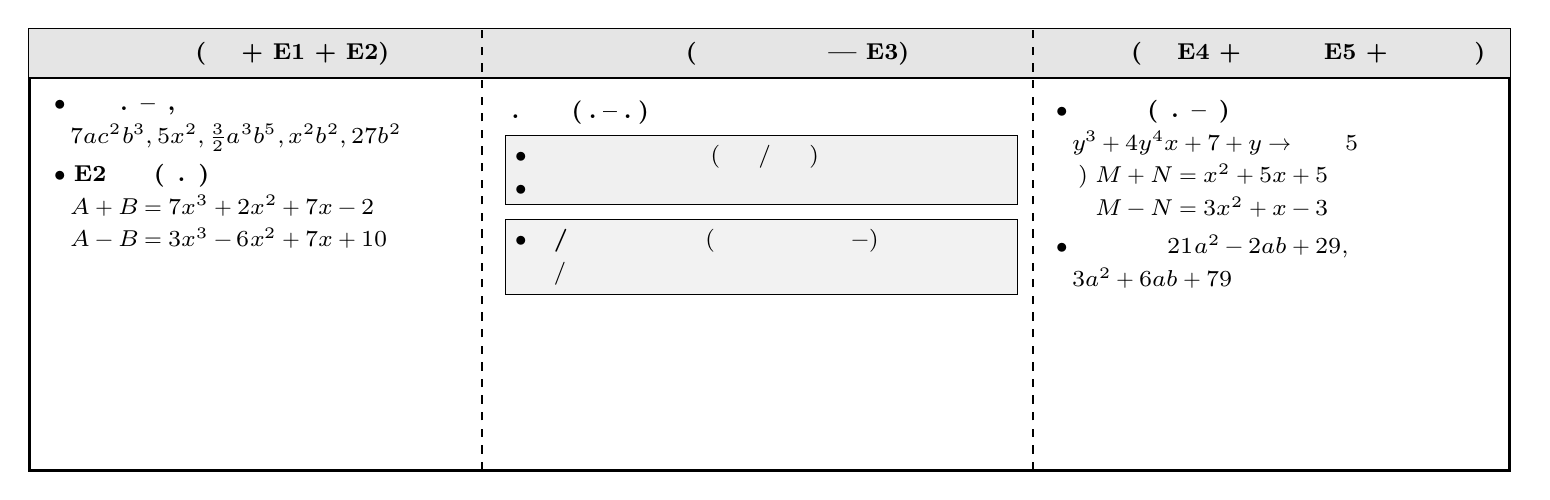
\begin{tikzpicture}[x=1cm, y=1cm, every node/.style={font=\fontsize{8.3pt}{11.8pt}\selectfont, text=black}]
  \draw[black, line width=1.1pt] (0,0) rectangle (18.8,5.60);
  \fill[gray!20] (0,4.98) rectangle (18.8,5.60);
  \draw[black, line width=0.7pt] (0,4.98) -- (18.8,4.98);
  \draw[black, dashed, line width=0.7pt] (5.75,0) -- (5.75,5.60);
  \draw[black, dashed, line width=0.7pt] (12.75,0) -- (12.75,5.60);

  \node at (2.875,5.29) {\textbf{ផ្នែកឆ្វេង (កំណែ + \en{E1} + \en{E2})}};
  \node at (9.25,5.29) {\textbf{ផ្នែកកណ្ដាល (ខ្លឹមសារគោលរក្សាទុក — \en{E3})}};
  \node at (15.775,5.29) {\textbf{ផ្នែកស្ដាំ (គំរូ \en{E4} + ប្រតិបត្តិ \en{E5} + កិច្ចការផ្ទះ)}};

  % Left
  \node[anchor=north west, text width=5.35cm] at (0.20,4.82) {%
    $\bullet$ \textbf{កំណែ ទំ.៥៤--៥៦, ៧២៖}\\
    \hspace*{0.2cm}$7ac^2b^3, 5x^2, \tfrac{3}{2}a^3b^5, x^2b^2, 27b^2$\\[2pt]
    $\bullet$ \textbf{\en{E2} ជួរឈរ (ទំ.៥៩)៖}\\
    \hspace*{0.2cm}$A+B = 7x^3 + 2x^2 + 7x - 2$\\
    \hspace*{0.2cm}$A-B = 3x^3 - 6x^2 + 7x + 10$
  };

  % Center
  \node[anchor=north west, text width=6.65cm] at (5.92,4.82) {%
    {\muol\fontsize{8.5pt}{12pt}\selectfont ២\enbf{.} ពហុធា \enbf{(}២\enbf{.}១\enbf{--}២\enbf{.}៣\enbf{)}}\\[3pt]
    \tikz\node[draw=black, fill=gray!12, inner sep=3.5pt, text width=6.25cm]{%
      $\bullet$ \textbf{ពហុធា៖} ផលបូកឯកធាមិនដូចគ្នា (ទ្វេធា/ត្រីធា)\\
      $\bullet$ \textbf{ដឺក្រេពហុធា៖} ដឺក្រេរបស់តួដែលមានដឺក្រេខ្ពស់ជាងគេ
    };\\[4pt]
    \tikz\node[draw=black, fill=gray!10, inner sep=3.5pt, text width=6.25cm]{%
      $\bullet$ \textbf{បូក/ដកពហុធា៖} លុបវង់ក្រចក (ប្ដូរគ្រប់សញ្ញាក្រោយ $-$) រួចបូក/ដកឯកធាដូចគ្នា
    };
  };

  % Right
  \node[anchor=north west, text width=5.8cm] at (12.92,4.82) {%
    $\bullet$ \textbf{លំហាត់គំរូ (ទំ.៥៨--៥៩)៖}\\
    \hspace*{0.2cm}$y^3+4y^4x+7+y \to$ ដឺក្រេ $5$\\
    \hspace*{0.2cm}ក) $M+N = x^2+5x+5$\\
    \hspace*{0.2cm}\phantom{ក) }$M-N = 3x^2+x-3$\\[2pt]
    $\bullet$ \textbf{ប្រតិបត្តិ ខ៖} $21a^2-2ab+29$,\\
    \hspace*{0.2cm}$3a^2+6ab+79$
  };
\end{tikzpicture}
\end{center}

\vspace{4pt}
\secstrip{២. ចម្លើយផ្ទៀងផ្ទាត់រហ័សសម្រាប់សន្លឹកកិច្ចការសិស្ស \enbf{(}ទំព័រ ១ និង ទំព័រ ២\enbf{)}}{\en{Answer Key}}

\begin{tcolorbox}[
  enhanced, sharp corners, colback=white, colframe=black,
  boxrule=0.8pt, boxsep=2pt, top=4pt, bottom=4pt, left=6pt, right=6pt
]
  \fontsize{9.0pt}{13.5pt}\selectfont
  $\bullet$ \textbf{ផ្នែក \en{E1}៖} \textbf{សិស្ស ខ} ត្រឹមត្រូវ ($2x^2-6x+2$) ព្រោះ $-(x^2+4x+5) = -x^2 - 4x - 5$ ។\\[2pt]
  $\bullet$ \textbf{ផ្នែក \en{E2}៖} \textbf{សកម្មភាព ១៖} $3y+2x+8$; ទ្វេធា និងត្រីធា; ដឺក្រេ $2$, ចុះ $5x^2-3x+11$ ។ \textbf{សកម្មភាព ២៖} $7a^2-4a+2$; $7x^3+2x^2+7x-2$ និង $3x^3-6x^2+7x+10$ ។\\[2pt]
  $\bullet$ \textbf{ផ្នែក \en{E4}៖} ១) ដឺក្រេ $3$, កើន $-4-k+k^2+2k^3$, ចុះ $2k^3+k^2-k-4$; អថេរ $x,y$, ដឺក្រេ $5$, ចុះ $4y^4x+y^3+y+7$; ២) $M+N = x^2+5x+5, \ M-N = 3x^2+x-3$ ។\\[2pt]
  $\bullet$ \textbf{ផ្នែក \en{E5}៖} ១) អថេរ $x,y$, $3$ តួ; ដឺក្រេ $3$; ២) $21a^2-2ab+29$ និង $3a^2+6ab+79$; ៣) សិស្ស ខ ($2x^2-6x+2$); ៤) \textbf{ជម្រើស \en{B}} ($3x^2+2x-3$); ៥) $3$ តួ ដឺក្រេ $4$ ។
\end{tcolorbox}

\vspace{4pt}
\secstrip{៣. ចម្លើយលម្អិតនៃកិច្ចការផ្ទះ \enbf{(}សម្រាប់ផ្ទៀងនៅដើមម៉ោងបន្ទាប់ ៥\enbf{.}២\enbf{.}៤\enbf{)}}{សៀវភៅគោល ទំ.៥៩, ៧២--៧៣}

\begin{tcolorbox}[
  enhanced, sharp corners, colback=white, colframe=black,
  boxrule=0.8pt, boxsep=2pt, top=4pt, bottom=4pt, left=6pt, right=6pt
]
  \fontsize{8.8pt}{13.2pt}\selectfont
  $\bullet$ \textbf{១) ប្រតិបត្តិទំ.៥៩ (គ)៖} $M+N = \mathbf{2xy^2 - 10xy - 19}$ \quad និង \quad $M-N = \mathbf{-xy^2 + 14xy + 13}$ ។\\[2pt]
  $\bullet$ \textbf{២) លំហាត់ \#4 (ទំ.៧២)៖} $A-B = (x^4+2x^4) + 3x^3 + (2x^2-x^2) + (-3x+x) + (1-3) = \mathbf{3x^4 + 3x^3 + x^2 - 2x - 2}$; \quad $B-A = -(A-B) = \mathbf{-3x^4 - 3x^3 - x^2 + 2x + 2}$ ។ \quad \textbf{\#5 ខ (ទំ.៧៣)៖} $\mathbf{7a^3b^2 - 4ab}$ ។
\end{tcolorbox}

\end{document}
